% =====================================================================
%  VI. Regime Map
%
%  Muc nay la cho "doi khung": tu "chung toi co loi the" sang "day la ranh
%  gioi". So 21/21/68 phai xuat hien nguyen ven, khong duoc chi ke 21 thang.
%  Nguon: results/nslkdd/regime_map_rows.csv, doi chieu ca 110 dong bang
%  runners/audit_c4.py muc E.
% =====================================================================



% Sinh boi runners/make_paper1_figures.py; caption doi chieu bang
% runners/audit_figures.py. File rieng cho tung hinh de \input DUNG CHO
% trong than bai -- float cua LaTeX chi troi VE SAU, khai bao het o cuoi
% tai lieu thi ca 9 hinh don xuong cuoi va tran vao danh muc tai lieu.

\begin{figure*}[t]
  \centering
  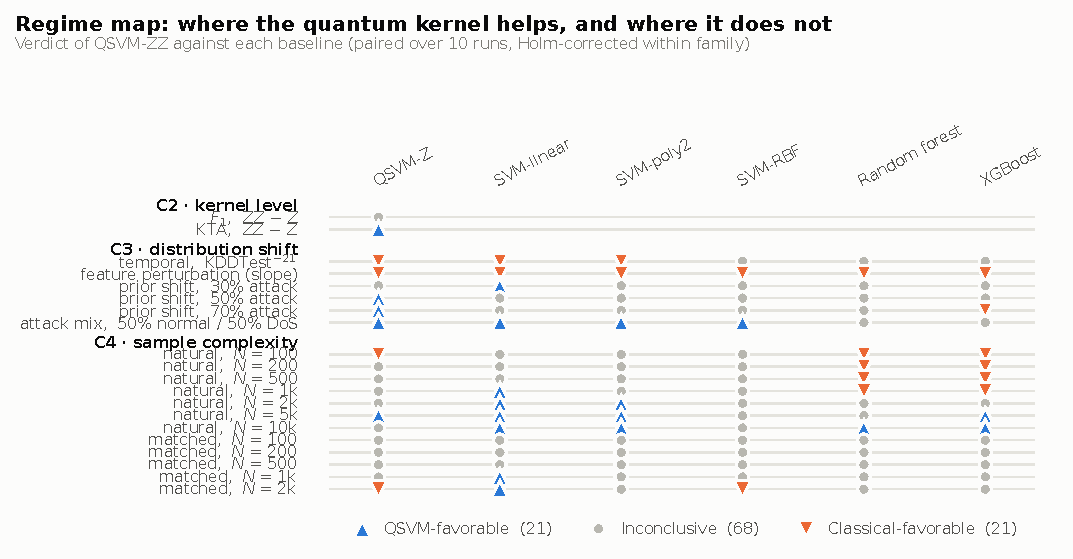
\includegraphics[width=\textwidth]{figs_revision/fig10_regime_map.pdf}
  \caption{%
    \textbf{Regime map: 110 controlled comparisons of \QSVM{} against six
    baselines.} Each cell is one paired comparison over ten runs, Holm-corrected
    within its baseline family (families of one to three; the $20$ cells
    against QSVM-\Zmap{} are uncorrected). Verdicts are encoded by both colour
    and glyph so the figure survives greyscale printing. The distribution is the
    result: $21$ favourable, $21$ classical-favourable, $68$ inconclusive within
    families; $17$, $15$ and $78$ under one Benjamini--Hochberg correction over
    all $110$ cells; and under Holm over all $110$ no cell survives. The seven
    C4-natural rows ($42$ cells) are the single-protocol block of
    Sec.~\ref{sec:regimemap}; the C2 and C3 rows are scored on a $300$- or
    $1000$-record test set. A single aggregate number would hide exactly the
    structure this paper is about.}
  \label{fig:regime-map}
\end{figure*}


Collecting every controlled comparison in one place gives the map in
Fig.~\ref{fig:regime-map}: $110$ cells, each a paired comparison between
\QSVM{} and one baseline under one condition, each carrying a Holm-corrected
verdict. Twenty-one favour the quantum kernel, twenty-one favour a classical
baseline, and sixty-eight are inconclusive. Two qualifications attach to that
count. The cells are corrected within families of one to three
(Sec.~\ref{sec:stats}); under a single Benjamini--Hochberg correction over all
$110$ cells the tally is $17$, $15$ and $78$, every cell that changes moving to
inconclusive and none changing side, and under Holm over all $110$ no cell
survives. And the cells come from two protocols that Sec.~\ref{sec:setup} says
are not interchangeable: $42$ cells from the natural prior on the full
KDDTest$^+$ partition (11 favourable, 9 unfavourable, 22 inconclusive) and $68$
from the rare-enriched pool (10, 12, 46), of which $30$ are scored on the full
partition and $38$ on a $300$-record or re-mixed $1000$-record test set. A
difference estimated on $300$ records and one estimated on $22{,}544$ do not
carry the same weight, and the reader who wants a single-protocol map should
read the natural-prior block on its own.

The balance of the first two numbers is the honest summary of this study. A
practitioner reading only the count would conclude that the quantum kernel is
neither better nor worse on average, and that conclusion would be correct and
useless. The map is worth more than its margin because the verdicts are not
distributed at random across conditions.

\subsection{Where it is worth the cost}
\revnote{rewrite}{The submitted forest plot had 9 rows; now 110 cells, each with $\Delta$, CI, $p$ and $d_z$ (R2-4).}
\begin{revbody}

Three conditions produce a favourable verdict, and they share a structure.

\emph{Enough data, natural prior.} At $N\geq5000$ under the natural class prior,
\QSVM{} is favourable against XGBoost and, at $N=10^{4}$, against the random
forest; it is favourable against the linear and poly-2 kernels from $N=1000$ and
$N=2000$. Below $N=2000$ the verdicts run the other way. The regime is bounded
on both sides: below it the kernel has too little data, and
Sec.~\ref{sec:res-width} shows that a wider circuit does not extend it upward.
It is also bounded from above by a model outside the paired protocol: every
favourable verdict here is against a baseline given the same four components,
and against XGBoost given all $122$ features the kernel reaches parity at
$N\geq5000$ (Table~\ref{tab:ref-arm}), while XGBoost on the full training
partition scores $0.804$, above any four-qubit model in this paper
(Sec.~\ref{sec:setup}). The regime is where the kernel is worth its cost
relative to a classical learner on the same embedding, not relative to the best
classical score available on the record.

\emph{Balanced binary composition.} On a $50/50$ Normal--DoS mixture the quantum
kernel is favourable against all four kernel baselines, with effect sizes up to
$3.02$. This is a C3 cell: models trained on the rare-enriched $N=1000$ pool
and scored on a re-mixed $1000$-record test set, so it lies outside the
natural-prior block and is not visible in the single-protocol reading. This is the condition under which quantum-kernel IDS results are most
often reported in the literature, and our numbers reproduce that impression;
which is part of why we report the other conditions too.

\emph{Rare-attack detection relative to tree ensembles.} At $N=10^{4}$ the
rare-class $F_{1}$ of \QSVM{} is $0.507$ against $0.334$ for XGBoost and $0.331$
for the random forest. If the deployment objective is rare-attack recall rather
than macro-averaged accuracy, the ranking changes substantially, though
SVM-RBF, at $0.585$, remains ahead of both.
\end{revbody}

\subsection{Where it is not}
\revnote{rewrite}{R2-4 observed that favourable regimes received full statistics and unfavourable ones only qualitative remarks; both sides now receive the same treatment.}
\begin{revbody}

\emph{Small training sets.} At $N\leq500$ the quantum kernel loses to both tree
ensembles at every size, by up to $0.081$ macro-$F_{1}$. No configuration we
tested recovers this.

\emph{Feature perturbation.} Six of six comparisons are classical-favourable
with effect sizes beyond $2.8$. The quantum kernel is the most perturbation-%
sensitive model in the study, which matters for a security application where
adversarial feature manipulation is the norm rather than the exception. Like
the balanced-composition result above, this is a C3 cell on the rare-enriched
pool and a $1000$-record test set, outside the natural-prior block; the two
clearest effect sizes in the map both come from that protocol.

\emph{Strong prior shift.} At a $70\%$ attack rate the comparison against
XGBoost is classical-favourable, and \QSVM{} degrades across the shift by
$0.032$ against $0.021$ for XGBoost. The submitted version presented this regime
as its strongest evidence; against strong tabular baselines it is evidence in
the opposite direction.

\emph{Wide circuits.} At $K=80$ and $n^{\ast}=8$, all $48$ comparisons are
classical-favourable. This is the sharpest boundary we found and the least
expected: it says the operating window is closed from above by the physics of
the feature map rather than by engineering limits that better hardware would
lift.

\emph{Any comparison against SVM-RBF on sample size.} Across the whole sweep, no
cell reaches corrected significance in the quantum kernel's favour. An RBF
kernel is the baseline this method does not clear.
\end{revbody}

\subsection{Reading the map}
\revnote{new}{New subsection, absorbing the ``decision rule'' of the submitted version.}
\begin{revbody}

Two properties of the map should govern how it is generalised.

First, the inconclusive cells are the majority, and they are informative. With
ten runs and Holm correction the smallest difference that reaches a verdict
anywhere in the map is $0.010$ macro-$F_1$, while differences as large as
$0.031$ remain inconclusive when their run-to-run spread is wide; the median
inconclusive cell sits at $0.014$. Most of the differences in this study are of
that order. A study reporting sharper verdicts on the same data with fewer
repetitions and no multiplicity control is not seeing more; it is resolving
less.

Second, the favourable regime is bounded on every axis we varied, and the
bounds are not far apart: $N \gtrsim 5000$ but not at a width beyond four to six
qubits, on NSL-KDD but not on UNSW-NB15 for the sample-size effect, and under
the natural prior, with the enriched prior untested at the sizes where the
regime lies. A method whose advantage is confined to a
box this small is not yet a practical instrument, and we do not present it as
one. What it is, on this evidence, is a phenomenon with a measurable boundary
and the boundary, being predicted by the circuit's phase-term count, is the
part most likely to hold beyond these two datasets.
\end{revbody}
